\section{Adding Data to the Data Package} \label{sec:adding-data}

In \autoref{sec:creating} of the User Guide, we stepped through the
process of creating a data package -- an entity that can contain data
objects and/or data object documentation. Data objects are most commonly
tables (delimited text files arranged in rows and columns) though Morpho
also supports documenting several image formats as well as data saved in
propriety formats such as Excel. Data documentation describes the data
object -- the columns and rows, the units used, etc. In this section we
will look at how to add data and data documentation to a package using
the Data Table wizard.

\subsection{Opening the Data Table Wizard} \label{sec:wizard-newtable}

The Data Table wizard (\autoref{fig:wizard-table-start}) helps users add
data and data documentation to a data package. The wizard steps through
the process of importing data (or manually creating it) and adding the
proper documentation. Note that you must complete the wizard. If you
exit before finishing, you will lose your changes.

\begin{figure}
  \centering
    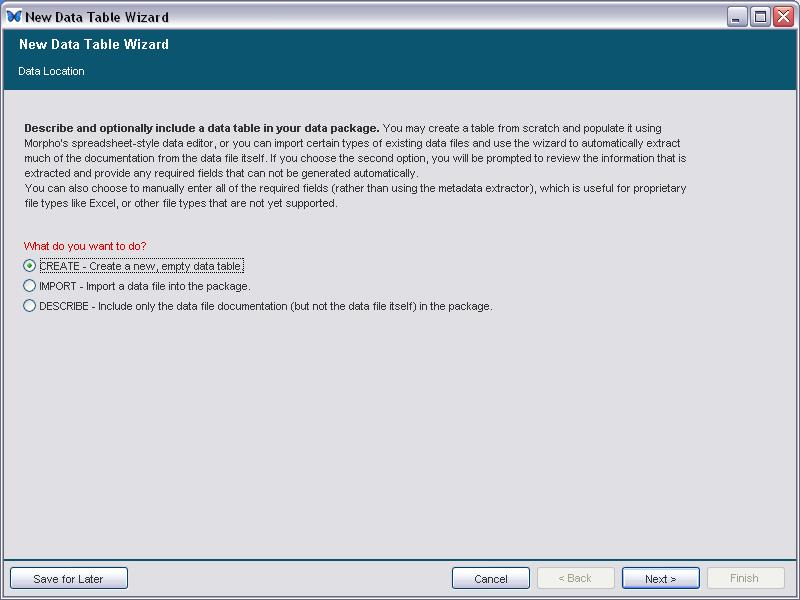
\includegraphics[width=0.7\textwidth]{images/wizard-table-start.jpg}
  \caption{The Data Table Wizard.}
  \label{fig:wizard-table-start}
\end{figure}

Users can choose to import an existing data table and
(optionally) extract metadata from it, or to document a data table
without including the data set itself in the package.

Fields labeled in red are required, and you cannot proceed to the next
step without first specifying the required values. 

To open the wizard and begin documenting a data table, do one of the
following:

\begin{itemize}
  \setlength{\parskip}{1pt}
  \item From the \nameref{sec:wizard-dp-summary} screen of the Data
    Package wizard (Step 15), click the ``or click here to finish this
    wizard and add a new data table now\ldots'' link.
  \item Open a data package and select ``Create/Import New Data
    Table\ldots'' from the \nameref{sec:menu-data} at the top of the
    Data Package screen.
\end{itemize}

On the first screen of the wizard, you must choose whether to  
\nameref{sec:table-create}, \nameref{sec:table-import}, or
\nameref{sec:table-describe} the data object:

\subsubsection{Create} \label{sec:table-create}

Document and then create a data table from scratch, populating it using
Morpho's spreadsheet-style data editor. 

If your data table does not yet exist, you may wish to create both the
documentation and data table using Morpho. The Data Table wizard leads
you through the required steps. See sections
\ref{sec:table-documenting}-\ref{sec:table-completing} for complete
instructions.

\subsubsection{Import} \label{sec:table-import}

Import a data table and (optionally) automatically extract documentation
from the data table to use in the metadata.

When you choose to import a data file, Morpho will (with your help)
locate the file on your computer, guide you through the documentation
process, and include the file as part of the data package
(\autoref{fig:wizard-table-import-options}). If your data set exists as
(or can be easily translated into) a delimited text file, you can
instruct Morpho to automatically extract certain documentation from the
data file (in which case, Morpho will extract table headers and other
information contained in the table and pre-populate the corresponding
wizard fields with information). When you import a delimited text file,
Morpho can also populate the wizard's spreadsheet editor with the
existing data fields.

\begin{figure}
  \centering
    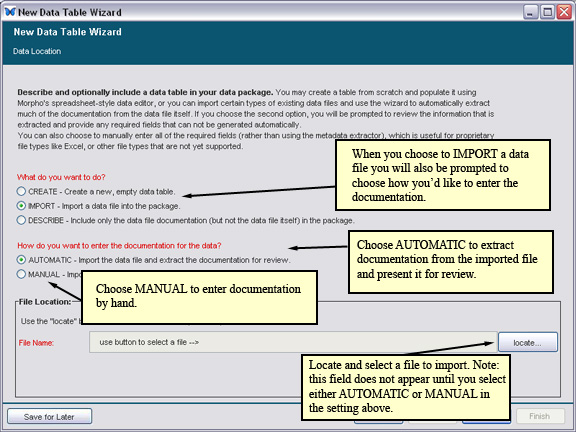
\includegraphics[width=0.7\textwidth]{images/wizard-table-import-options.jpg}
  \caption{Importing data files with the Data Table wizard.}
  \label{fig:wizard-table-import-options}
\end{figure}

If you choose to manually enter documentation, the Data Table wizard
will take you through the steps outlined in
\autoref{sec:table-documenting} and \autoref{sec:table-completing}. If
you choose to automatically extract and import documentation, the Data
Table wizard first displays your data table for review. We look at the
process of importing documentation more closely in the
\nameref{sec:table-importing-documentation} section.

\subsubsection{Describe} \label{sec:table-describe}

Document the data, but do not include the data in the data package.

If you choose to describe your data, the Data Table wizard will step you
through the process of providing documentation for it. Describing data
is useful for documenting the data for yourself, as well as for telling
others about the data (if the data package is saved to a network)
without sharing the data set itself (Note that you can also control
access to the data table by \hyperref[sec:edit-table-access]{setting
access restrictions} for it). You might also choose this option if the
data are not available in digital form, or if the data are available at
an online URL.

\subsection{Documenting the Data Table} \label{sec:table-documenting}

The first few screens of the Data Table wizard collect
\nameref{sec:table-file-info}, \nameref{sec:table-info}, and
\nameref{sec:table-attribute-info}.

\subsubsection{Data File Information} \label{sec:table-file-info}

Once you have selected how you would like to add a data table to the
package (by creating, importing, or describing it), the Data Table
wizard requests information about the format of the data file
(\autoref{fig:wizard-table-fileinfo}).

The instructions in this section are for working with tabular data
(e.g., simple delimited text). For more information about working with
non-text or proprietary formatted files, see
\nameref{sec:table-other-types}.

\begin{figure}
  \centering
    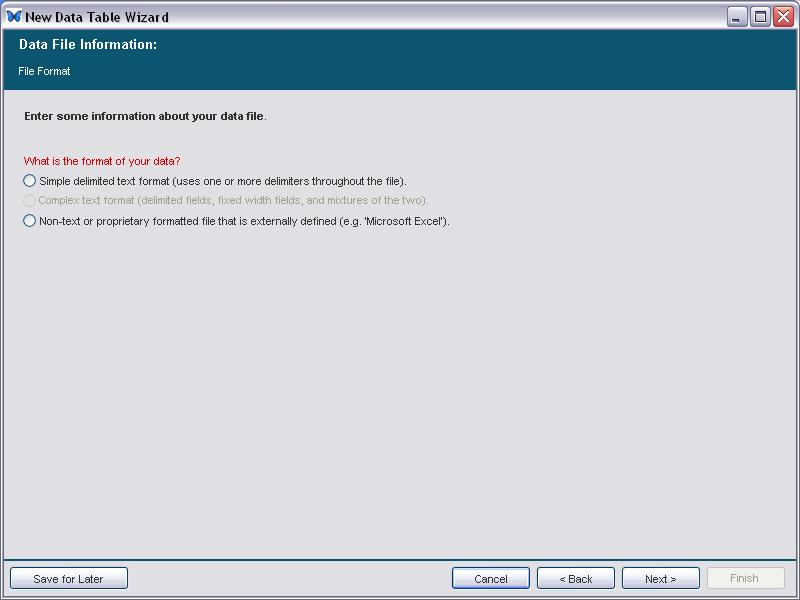
\includegraphics[width=0.7\textwidth]{images/wizard-table-fileinfo.jpg}
  \caption{The Data Table wizard: specifying file format information.}
  \label{fig:wizard-table-fileinfo}
\end{figure}

After selecting a data file format, the Data Table wizard requests
additional details about that format
(\autoref{fig:wizard-table-fileformat})

\begin{figure}
  \centering
    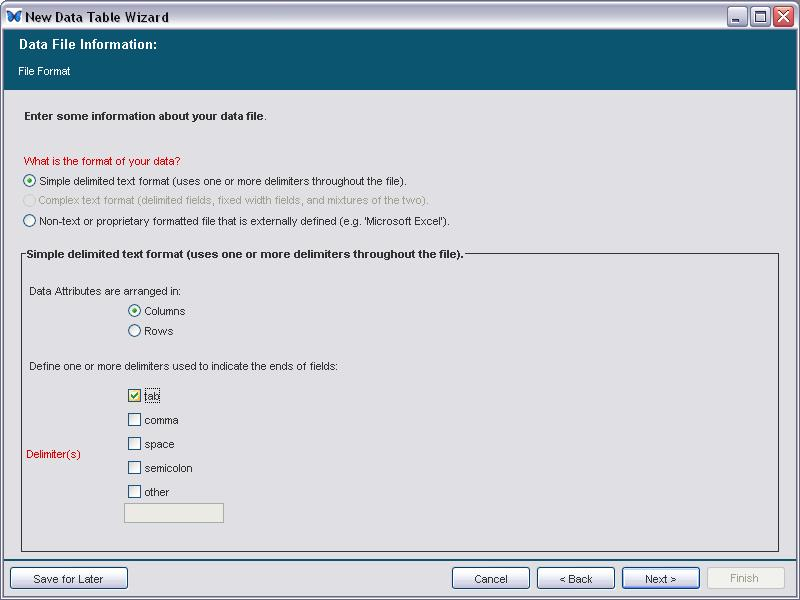
\includegraphics[width=0.7\textwidth]{images/wizard-table-fileformat.jpg}
  \caption{Adding details about the data format in the Data Table
    wizard.}
  \label{fig:wizard-table-fileformat}
\end{figure}

A delimiter -- the character used to indicate the separation of each
data field in your table -- is required. Often, the delimiter is a
comma. If you are importing a data file and do not know what delimiter
it uses, open the file and check to see how the table values are
separated. You should also specify whether attributes are arranged in
columns (i.e., the headers run across the top of the table) or rows (the
headers run down the left side of the table). 

\subsubsection{Data Table Information} \label{sec:table-info}

Data packages may contain any number of data tables. In order to clearly
identify each, the Data Table wizard prompts you to specify a table
name, description, and attribute documentation
(\autoref{fig:wizard-table-describe}).

\begin{figure}
  \centering
    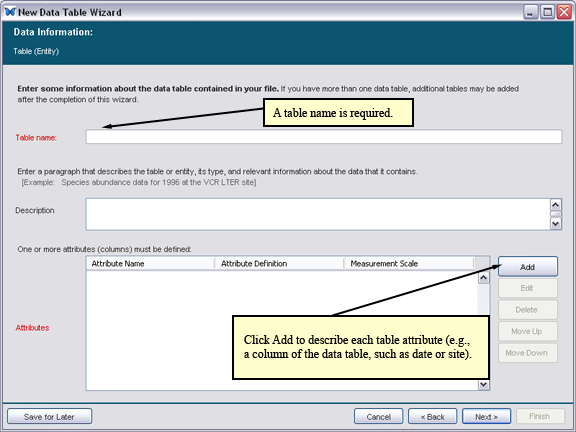
\includegraphics[width=0.7\textwidth]{images/wizard-table-describe.jpg}
  \caption{Adding data table information with the Data Table wizard.}
  \label{fig:wizard-table-describe}
\end{figure}

A table name is required, as well as at least one attribute definition
(we recommend that you document all attributes). The table name is used
to identify the table, and should be short but still uniquely identify
the table. An attribute is usually a column of the data table, such as
date or site. For example, a definition for a site attribute would
clarify what the values mean (e.g., ``1 of 5 sites around Lake Erie'').
Though a table description is not required, we recommend that you
briefly describe the table and provide information about the data it
contains (e.g., ``Species abundance data for 1996 at the VCR LTER site'')
to document the overall meaning of the table.

Click the Add button to open the Define Attribute screen and begin
documenting the table attributes (\autoref{fig:wizard-table-attribute}). We will look at this
screen in more detail in the next section.

\begin{figure}
  \centering
    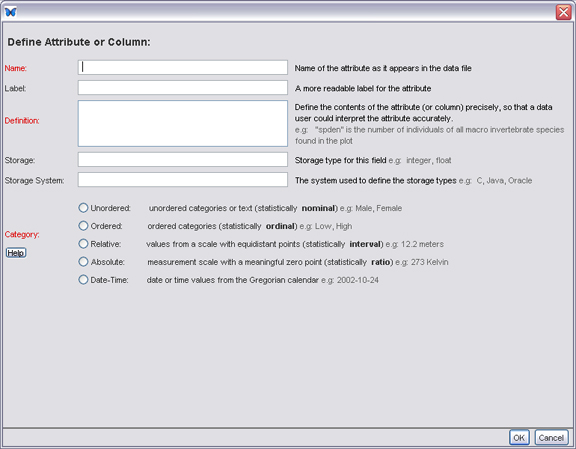
\includegraphics[width=0.7\textwidth]{images/wizard-table-attribute.jpg}
  \caption{Define table attributes. We look at each of these fields in
    more detail in the following section.}
  \label{fig:wizard-table-attribute}
\end{figure}

\subsubsection{Data Attribute Information} \label{sec:table-attribute-info}

Specifying data attribute information helps you and other people using
your data interpret the data accurately. For example, if a column of
data is titled ``spden'' -- a term that might be familiar to your
research team, but not other scientists who may later join it (or view
your data on the network) -- you can clarify the meaning when you define
the table attributes. For each attribute (i.e., column of data), you
have an opportunity to document the name as it appears in the data
table, a label that may more clearly reflect the value, a definition
that further elucidates the meaning of the value, storage information,
and category information. Category information, which documents the
attribute's measurement scale, is required.

\begin{itemize}
  \setlength{\parskip}{1pt}
  \item \nameref{sec:table-attribute-name}
  \item \nameref{sec:table-attribute-name}
  \item \nameref{sec:table-attribute-name} (\nameref{par:cat-unordered},
    \nameref{par:cat-ordered}, \nameref{par:cat-relative},
    \nameref{par:cat-absolute}, \nameref{par:cat-datetime})
\end{itemize}

Although the Data Table wizard requires that you document only one table
attribute, we strongly recommend that you document all table attributes.

\subsubsection*{Name, Label, and Definition}
\label{sec:table-attribute-name}

The Name, Label, and Definition fields identify the name and contents of
the data column (\autoref{fig:wizard-table-attribute-name}). The Name
field is required. If you are importing a data table that contains a
header row, the value should match the headers used in the data file.
Morpho will detect the headers if you chose to extract metadata
automatically, otherwise you will have to enter the names manually. If
you are creating a data table, the name value will be used to identify
the data column. The Label field is optional, but we recommend that you
specify a more readable column name if the original name is difficult to
interpret. The Definition, which is also required, further clarifies the
meaning of the data column. The Definition is probably the most
important part of defining the attribute because it provides information
that helps future data users understand what the attribute means or
represents.

\begin{figure}
  \centering
    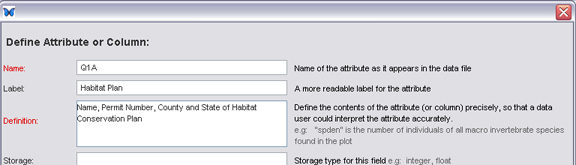
\includegraphics[width=0.7\textwidth]{images/wizard-table-attribute-name.jpg}
  \caption{Example values for the Name, Label, and Definition fields. In
    this example, the data column in the data file is titled Q1A. The
    Label and Definition fields clarify the value.}
  \label{fig:wizard-table-attribute-name}
\end{figure}

\subsubsection*{Storage and Storage System}
\label{sec:table-attribute-storage}

The Storage and Storage System fields help identify the structural type
of the column values. Though not required, specifying this information
helps data users know how your data are stored. Some common types
include string, Boolean, integer, float, long, double, matrix, object,
scalar, and array. How each structural type is defined depends on the
system used (Java, Oracle, etc). 

\subsubsection*{Category}
\label{sec:table-attribute-category}

Categories describe how the data are measured, what measurement scale
they use (\autoref{tab:attr-categories}), and how values are enumerated
and defined on that scale. Selecting the proper measurement scale is
critical because the scale determines the types of statistics you can
use to analyze your data. The measurement scale also dictates the type
of metadata needed to describe your data set (for example, categorical
data never have a ``unit'' of measurement). When you select a category,
the Data Table wizard automatically prompts you to enter only the
relevant information.

The categories used in the Data Table wizard are based on Steven's
original typology (Stevens, SS (1946). On the theory of scales of
measurement. Science, 103(2684):677), with the addition of ``Date-Time''
for purely pragmatic reasons (we need to distinguish date-time values in
order to collect certain essential metadata about date and time
representation). In this section, we will look more closely at each
measurement scale and when it should be used. It is important to keep in
mind that a given type of data may fall under more than one measurement
scale (for example, values using an ordered scale such as ``strongly
agree, agree, disagree'', also represent categories that can be described
by an unordered scale). This is because each measurement scale is a
superset of the one beneath it in Table 7.1 (i.e., ordinal data are also
nominal, interval data are also ordinal and nominal, and ratio data are
also interval, ordinal, and nominal). When selecting a category, select
the most restrictive category (i.e., closer to the bottom of the table)
that still accurately describes the attribute's data.

After you have chosen a category, the Data Table wizard prompts you to
describe the units, number types, and other details about the categories
themselves.  

\begin{table}[htbp]
  \centering
  \begin{tabular}{|c|m{0.7\textwidth}|}
  \hline
  \textbf{Category} & \textbf{Description} \\
  \hline
  \nameref{par:cat-unordered} &
    The unordered, or nominal, scale places values into named
    categories. The different values within a set are unordered. Some
    examples of unordered scales include gender (Male/Female) and
    marital status (single/married/divorced). Text fields should be
    classified as nominal. \\
  \hline
  \nameref{par:cat-ordered} &
    The ordered, or ordinal, scale places values in a set order. Ordinal
    data show a particular value's position relative to other values,
    such as ``low, medium, high, etc.'' The ordinal scale doesn't
    indicate the distance between each item. Some examples of ordered
    scales include level of agreement (Strongly agree, Agree, Disagree,
    Strongly disagree), or age class (Juvenile, Sub-adult, Adult). \\
  \hline
  \nameref{par:cat-relative} &
    The relative, or interval, scale uses a measurement scale of
    equal-sized units (e.g., degrees Celsius). The scale starts from an
    arbitrary point (not a meaningful zero), and so there is no concept
    of 'zero' of the measured quantity. Consequently, ratios of relative
    values are not meaningful. Some examples of relative scales include
    the Celsius temperature scale and the Fahrenheit temperature scale. \\
  \hline
  \nameref{par:cat-absolute} &
    The absolute, or ratio, scale is an interval scale with a meaningful
    zero point. The ratio scale begins at a true zero point that
    represents an absolute lack of the quality being measured. Thus,
    ratios of values are meaningful. Examples of absolute, or ratio,
    scales include elevation (measured from sea-level), height, and the
    Kelvin temperature scale. \\
  \hline
  \nameref{par:cat-datetime} &
    Examples of date-time values are '2003-05-05', '1999/10/10', and
    '2001-10-10T14:23:20.3'. \\
  \hline
  \end{tabular}
  \caption{The five measurement scales used in Morpho. Each scale is a
    superset of the ones beneath it in the table.}
  \label{tab:attr-categories}
\end{table}

\paragraph{Unordered (nominal)} \label{par:cat-unordered}

The unordered, or nominal, scale places values into named categories.
The different values within a set are unordered. Some examples of
unordered scales include gender (Male/Female) and marital status
(single/married/divorced). Text fields (e.g., names of study sites or
U.S. telephone numbers) should be classified as nominal.

When ``Unordered'' is chosen, the Data Table wizard prompts you to
choose whether the values are ``enumerated values belonging to a
predefined list'' (e.g., single/married/divorced), or if they are ``text
values.'' Text values can be free-form or can match a pattern that is
specified in the wizard as well. 

If you choose ``Enumerated values,'' you will be required to define the
code used by the values so that users know what each represents (e.g.,
M=``male''; F=``female'', etc). To define codes manually in the Data
Table Wizard, select ``Codes are defined here'' under Location
(\autoref{fig:wizard-table-attribute-codedefs-manual}). You can also
choose to import codes from an existing data table by selecting ``Codes
are imported from another table'' under Location
(\autoref{fig:wizard-table-attribute-codedefs-import}).

\begin{figure}
  \centering
    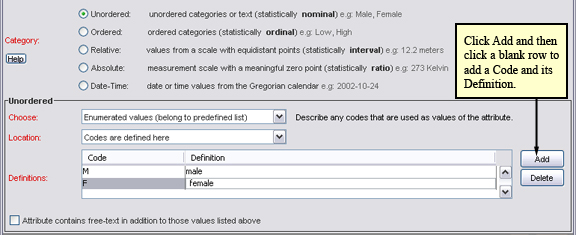
\includegraphics[width=0.7\textwidth]{images/wizard-table-attribute-codedefs-manual.jpg}
  \caption{Select ``Codes are defined here'' as the Location setting to
    define codes in the wizard.}
  \label{fig:wizard-table-attribute-codedefs-manual}
\end{figure}

\begin{figure}
  \centering
    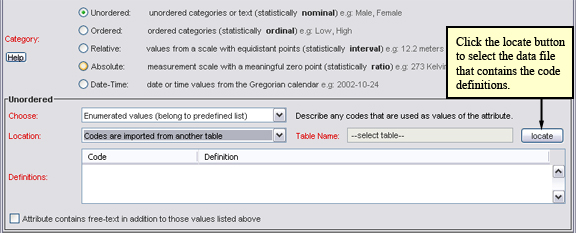
\includegraphics[width=0.7\textwidth]{images/wizard-table-attribute-codedefs-import.jpg}
  \caption{Select ``Codes are imported from another table'' under the
    Location setting to select code definitions from the imported data
    table (or to import the definition table later).}
  \label{fig:wizard-table-attribute-codedefs-import}
\end{figure}


Clicking the ``locate'' button brings you to the screen that allows you
to import the codes later (``Import the definitions table into Morpho
later''). If you are importing a data table and the codes and their
definitions are already contained in it, you can also choose to select
the codes/definitions from the table
(\autoref{fig:wizard-code-definition}). When ``The definitions table has
already been included in this package'' is selected, the Data Table
wizard displays the contents of the included data tables, allowing you
to select the column that contains the code and the column that contains
the definition. Click OK to update the ``Definitions'' setting with the
selected codes and definitions.

Note the check-box at the bottom of the Define Attribute or Column
screen. Check this box if your columns of data contain free-text, such
as notes, in addition to the defined codes you provide in the
``Definitions'' table. 

\begin{figure}
  \centering
    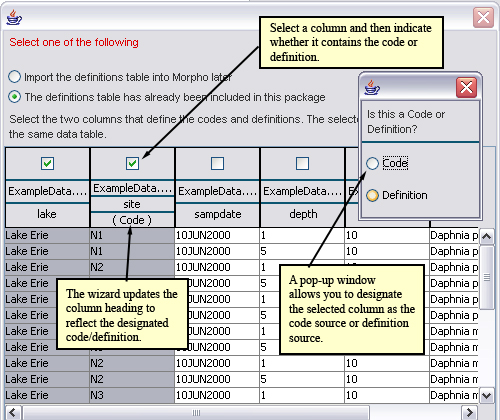
\includegraphics[width=0.7\textwidth]{images/wizard-code-definition.jpg}
  \caption{Selecting codes and definitions from the imported data
    table.}
  \label{fig:wizard-code-definition}
\end{figure}

If the data in the attribute or column are unordered text values, choose
``Unordered'' from the ``Category'' list, and choose ``Text values
(free-form or matching a pattern)'' from the drop-down menu next to
``Choose''. The wizard prompts you to define the text values, and
provide the name of their source, if applicable
(\autoref{fig:wizard-table-attribute-text-values}). You can optionally
define the pattern of the text values by clicking the ``Add'' button,
and typing the pattern into the ``Pattern(s)'' table. 

\begin{figure}
  \centering
    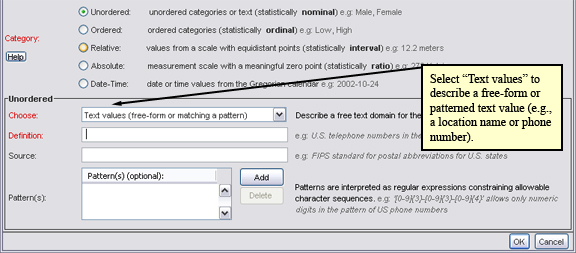
\includegraphics[width=0.7\textwidth]{images/wizard-table-attribute-text-values.jpg}
  \caption{Select ``Text values (free-form or matching a pattern) to
    identify unordered text values. You are required to specify a
    definition for unordered text values.}
  \label{fig:wizard-table-attribute-text-values}
\end{figure}

\paragraph{Ordered (ordinal)} \label{par:cat-ordered}

Ordered data show a particular value's position relative to other
values, such as ``low, medium, high.'' The ordinal scale does not
indicate the distance between each item. Examples of ordered scales
include level of agreement (Strongly agree, Agree, Disagree, Strongly
disagree), or age class (Adult, Sub-adult, Juvenile).

If the data column contains data measured on an ordered scale, select
``Ordered'' as the attribute category. The user interface for defining
ordered values is the same as the one for defining unordered values. See
\nameref{par:cat-unordered} for more information about the required
fields.

\paragraph{Relative (interval)} \label{par:cat-relative}

The relative, or interval, scale uses a measurement scale of equal-sized
units (e.g., degrees Celsius). The scale starts from an arbitrary point
(not a meaningful zero), and so there is no concept of 'zero' of the
measured quantity. Consequently, ratios of relative values are not
meaningful. For example, one cannot infer that someone with a score of
80 on an ecology test knows twice as much ecology as someone who scores
40 on the test, or that an object at 40 degrees C has twice the kinetic
energy as an object at 20 degrees C. Some example of relative scales
include the Celsius temperature scale and the Fahrenheit temperature
scale.

NOTE: To make ratio comparisons legitimate, interval values must first
be converted to \hyperref[par:cat-absolute]{absolute values} (in
general, absolute scales are much more common). For example, convert
Celsius temperatures (relative values) to Kelvin (an absolute scale with
a real 0 point). An object at 40 degrees C is 313.15 degrees Kelvin and
an object at 20 degrees C is 293.15 degrees Kelvin. The first object has
approximately 1.07 times more kinetic energy than the second (not twice
as much).

If the data column contains data measured on a relative scale, select
``Relative'' as the attribute category. The Data Table wizard updates to
include fields for specifying the measurement unit and precision, as
well as the type of number used (e.g., natural or integer)
(\autoref{fig:wizard-table-define-new-unit}).

\begin{figure}
  \centering
    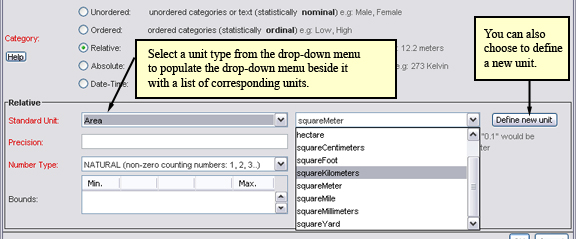
\includegraphics[width=0.7\textwidth]{images/wizard-table-define-new-unit.jpg}
  \caption{Defining units and precision for a relative measurement
    scale.}
  \label{fig:wizard-table-define-new-unit}
\end{figure}

When specifying a unit, first select the unit type (i.e., measurement
category) from the drop-down menu beside ``Standard Unit''. Each unit
type contains units for measuring it. For example, the ``Speed'' unit
type includes units such as ``metersPerSecond'' and ``milesPerHour.''
Once you select a unit type, the drop-down menu to the right will
automatically be populated with corresponding units.

If the unit used by your data does not appear in the unit drop-down
menu, you can define a new unit to represent it. For example, if your
data includes acceleration measurements (the change in velocity over
time, expressed by the \href{http://en.wikipedia.org/wiki/SI}{SI unit}
$m/s^2$) for thirteen-meter intervals instead of one-meter intervals, you
would define a new unit thirteenMetersPerSecondSquared (as opposed to
the existing measurement, metersPerSecondSquared). To do this, click the
``Define New Unit'' button and enter a name and description for the unit
(\autoref{fig:wizard-table-attribute-newunit-name}). 

\begin{figure}
  \centering
    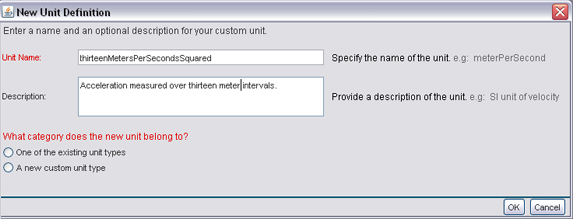
\includegraphics[width=0.7\textwidth]{images/wizard-table-attribute-newunit-name.jpg}
  \caption{Entering a new unit name and description.}
  \label{fig:wizard-table-attribute-newunit-name}
\end{figure}

Once you have created a unit name and description, specify whether the
new unit belongs to an existing unit type, or to a new custom unit type.
Please note that at this time, the interface for defining a new custom
unit type is incomplete. See the \hyperref[box:custom-units]{text box}
for more information. In the acceleration example presented in
\autoref{fig:wizard-table-attribute-newunit-name}, the new unit belongs
to an existing type (Acceleration). Select the ``One of the existing
unit types'' radio button
(\autoref{fig:wizard-table-attribute-newunit-existingtype}) and then
select the unit type. You must also specify the Multiplier (in this case
.0769) that can be used to convert the custom unit ($13m/s^2$) to the SI
unit ($m/s^2$). 

\begin{figure}
  \centering
    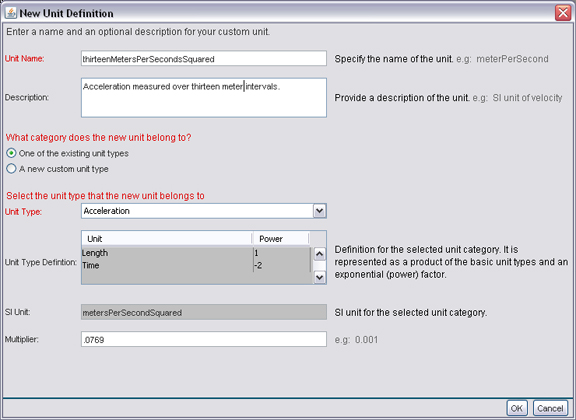
\includegraphics[width=0.7\textwidth]{images/wizard-table-attribute-newunit-existingtype.jpg}
  \caption{Defining a new unit based on one of the existing unit types.
    The example above shows the fields that appear if you are defining a
    unit of type ``Acceleration''.}
  \label{fig:wizard-table-attribute-newunit-existingtype}
\end{figure}

\begin{shaded}
  \label{box:custom-units}
  \emph{\textbf{A Note about Custom Unit Types}}

  Currently, you cannot use the Morpho wizard to create a new custom
  unit type because the interface does not permit you to associate a new
  SI unit with that unit. We are working to enable this functionality,
  which will ship with the next release of Morpho.

  \begin{center}
      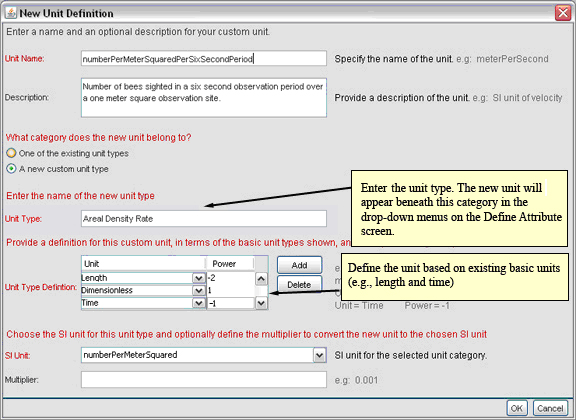
\includegraphics[width=0.7\textwidth]{images/wizard-table-attribute-newunit-newtype.jpg}
  \end{center}

  A custom unit type is required when the new unit does not belong to an
  existing unit type. For example, if your data set contains
  measurements for ``number of bees sighted per square meter per six
  seconds,'' you would have to define a new unit type to represent that
  measurement. This new unit for measuring bees is a custom type,
  ``Areal Density Rate.'' An example of a new unit that belongs to an
  existing unit type is ``bees per 10 square meters,'' where you simply
  wish to apply a multiplier to the existing unit (number per meter
  squared, an ``Areal Density''). Note that you can define new units
  that belong to existing types.

  %\begin{figure}
  %  \centering
  %    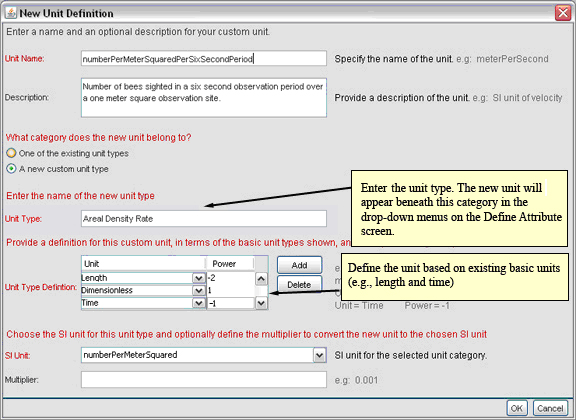
\includegraphics[width=0.7\textwidth]{images/wizard-table-attribute-newunit-newtype.jpg}
  %  \caption{An example of a new custom unit. NOTE THAT CURRENTLY,
  %    MORPHO DOES NOT SUPPORT DEFINING A NEW CUSTOM UNIT TYPE}
  %  \label{fig:wizard-table-attribute-newunit-newtype}
  %\end{figure}

  To define the new unit, create a definition using basic units (e.g.,
  ``length'' and ``time'') and specify an exponential factor (e.g., 1 or
  -1). To define our measurement ``number of bees sighted per square
  meter per six seconds'', click the Add button and select ``Length''
  from the Unit drop-down menu. Set the Length unit's power to -2. Click
  ``Add'' again and choose ``Time'' from the Unit drop-down menu. Set
  the Time unit's power to -1. Click ``Add'' a third time and choose
  ``Dimensionless'' from the drop-down menu. Set the Dimensionless
  unit's power to 1. Putting those three units together according to the
  indicated powers gives you a new unit of (number)/(time * square
  meters). 

  You must also specify the \href{http://en.wikipedia.org/wiki/SI} {SI
  Unit} that corresponds to the new unit. The SI unit for a derived type
  is the base SI type for each part of the derivation.  For example, the
  base SI unit for length is meter, and for time is second.  The SI unit
  for velocity (distance/time) would therefore be $m/s$.  The SI unit that
  represents the unit we derived to represent bees per square meter per
  six seconds is $1/sm^2$. If known, you can also provide the
  conversion factor that converts your unit to the SI unit (in the
  Multiplier field).
\end{shaded}

After choosing or defining the unit, specify the precision of the data
in the Precision field (\autoref{fig:wizard-table-define-new-unit}). For
example, if the attribute is measured in meters, a precision of ``0.1''
would be interpreted as precise to the nearest 1/10th of a meter. You
must also choose the number type used by the data: natural, whole,
integer, or real (\autoref{tab:number-types}). The four number types in
the drop-down menu are not discrete classes – some overlap. Remember to
choose the type that most specifically and accurately describes the data
in the attribute or column you are defining. Optionally, you can provide
the minimum and maximum values for the data column by clicking the Add
button beside the Bounds field at the bottom of the screen. 

\begin{table}[htbp]
  \centering
  \begin{tabular}{|c|m{0.7\textwidth}|}
  \hline
  \textbf{Number Type} & \textbf{Description} \\
  \hline
  Natural numbers &
    Natural numbers are positive and non-zero counting numbers (i.e.,
    non-fractions), such as 1, 2, 3, and so on. They cannot be negative
    or zero. When thinking of counting numbers, think about counting a
    basket of oranges, or counting something using your fingers
    (although natural numbers can be larger than ten). There are no
    fractions of oranges or fractions of fingers (hopefully!), and there
    are no negative numbers of oranges or negative numbers of fingers.
    Natural numbers are one type of whole numbers. \\
  \hline
  Whole numbers &
    Whole numbers are just like natural numbers, except zero is included
    in the set of whole numbers, and therefore whole numbers are
    positive counting numbers and zero: 0, 1, 2, 3, and so on. Just like
    natural numbers, they cannot be fractions or negative. Whole numbers
    are a type of integer, and they include natural numbers. \\
  \hline
  Integer numbers &
    Integers are just like whole numbers, except negative counting
    numbers are included in this set. Therefore integers are positive
    and negative counting numbers and zero, such as -3, -2, -1, 0, 1, 2,
    3, and so on. Just like whole and natural numbers they cannot be
    fractions. Integers are a type of rational numbers, and they include
    whole numbers and natural numbers. \\
  \hline
  Real numbers &
    Real numbers are the broadest set of numbers. They can be negative
    and positive fractions and counting numbers, and can include zero.
    Therefore a list of numbers like the following would be a set of
    real numbers: -1/2, -0.25, 3.14, 0, 1, -25, 5/8, and so on. As you
    can see from this list of examples, real numbers include integers,
    whole numbers, and natural numbers. \\
  \hline
  \end{tabular}
  \caption{The four number types used by data attributes.}
  \label{tab:number-types}
\end{table}

\paragraph{Absolute (ratio)} \label{par:cat-absolute}

The absolute, or ratio, scale is an interval scale with a meaningful
zero point. The ratio scale begins at a true zero point that represents
an absolute lack of the quality being measured. Thus, ratios of values
are meaningful. For example, an object that is 100 meters above sea
level is twice as high as an object that is 50 meters above sea level
(where sea level is the zero point). Also, an object at 300 degrees
Kelvin has three times the kinetic energy of an object at 100 degrees
Kelvin (where absolute zero (no motion) defines the zero point of the
Kelvin scale). Examples of absolute, or ratio, scales include elevation,
height, area, and the Kelvin temperature scale. (Note: Absolute scales
are much more common than \hyperref[par:cat-relative]{relative ones}).

If the data column contains data measured on an absolute scale, select
``Absolute'' as the attribute category. The user interface for defining
absolute values is the same as the one for defining relative values. See
\nameref{par:cat-relative} for more information about the required
fields.

\paragraph{Date-Time} \label{par:cat-datetime}

Date and time values can be represented using several distinct notations
(e.g., '2003-05-05', '1999/10/10', and '2001-10-10T14:23:20.3'), and the
metadata must document the format used by the data in order to clearly
communicate the values.

If the data column contains data measured on a date-time scale, select
``Date-Time'' as the attribute category. The Data Table wizard updates to
include fields for specifying the date format and precision
(\autoref{fig:wizard-table-attribute-datetime}).

\begin{figure}
  \centering
    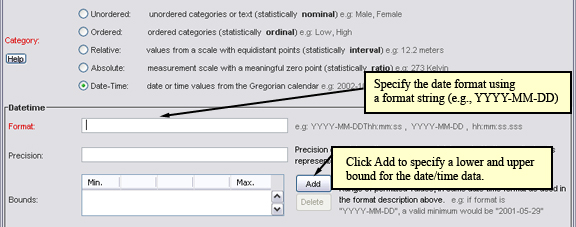
\includegraphics[width=0.7\textwidth]{images/wizard-table-attribute-datetime.jpg}
  \caption{Specifying a date format using format strings. Optionally,
    you can specify the precision as well as an upper and lower bound
    for the data.}
  \label{fig:wizard-table-attribute-datetime}
\end{figure}

Type the format of the date and/or time in the field next to ``Format''
using an ISO 8601  format string like the examples given to the right of
the field. For additional examples of date format strings, please see
the \href{http://knb.ecoinformatics.org/software/eml/eml-2.1.1/eml-coverage.html}
{EML documentation}. You can also provide the precision of the date
and/or time format and indicate the upper and/or lower bounds of the
date and/or time using the ``Bounds'' table at the bottom of the screen. 

\begin{shaded}
  \textbf{NOTE} Date and time values in the Gregorian calendar are very
  strange to use in calculations in that they have properties of both
  relative and absolute scales. They also have some properties that do
  not conform to the relative scale because of the adjustments that are
  made to time to account for the variations in the period of the Earth
  around the sun (e.g., leap years). While the Gregorian calendar has a
  meaningful zero point, it would be difficult to say that a value taken
  on midnight January 1, 1000 is twice as old as a value taken on
  midnight January 1, 2000 because the scale has many irregularities in
  length in practice. However, over short intervals the scale has
  equidistant points based on the SI second, and so can be considered
  relative for some purposes, especially with respect to measuring the
  timing of short-term ecological events.
\end{shaded}

\subsection{Completing the Wizard} \label{sec:table-completing}

After you have finished stepping through the screens described in
\autoref{sec:table-documenting}, you will have added a description of
ONE of the attributes (i.e., columns of data) in the data table. The
described attribute will appear in the Data Information screen
(\autoref{fig:wizard-table-info}). 

To describe another attribute, click ``Add'', and repeat the wizard steps
for the new attribute. Note that if you choose to extract documentation
automatically, you will not see this screen. For more information about
extracting documentation automatically, please see the
\nameref{sec:table-importing-documentation} section.

\begin{figure}
  \centering
    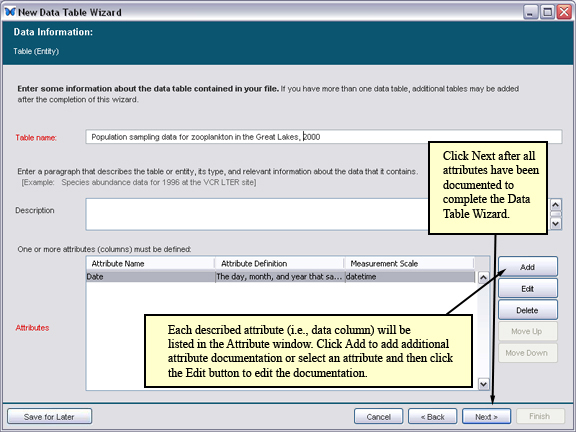
\includegraphics[width=0.7\textwidth]{images/wizard-table-info.jpg}
  \caption{Documented data attributes are listed in the Attributes
    window. Click Add to document addtional attributes.}
  \label{fig:wizard-table-info}
\end{figure}

After you have documented all table attributes, click the Next button to
view the final screen of the New Data Table wizard
(\autoref{fig:wizard-table-finish}).

\begin{figure}
  \centering
    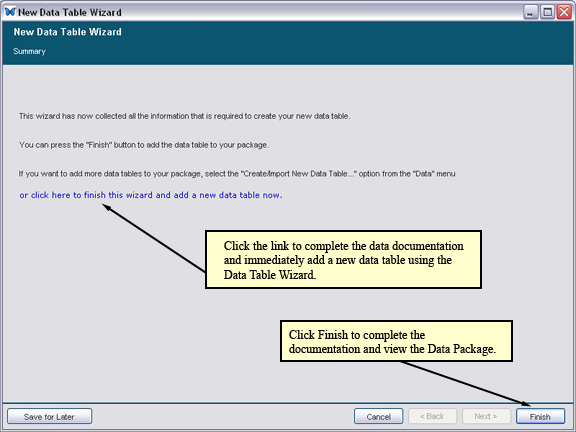
\includegraphics[width=0.7\textwidth]{images/wizard-table-finish}
  \caption{To complete the Data Table wizard, click Finish or the
    ``click here to finish this wizard and add a new data table now''
    link.}
  \label{fig:wizard-table-finish}
\end{figure}

Click ``Finish'' to finish documenting the data table, and then save the
data package to save your changes. 

If you chose to create a data table when you started the wizard, Morpho
will display the data package containing your new table documentation
and an empty data table after you click Finish. Type data directly into
the empty columns, or copy and paste data from elsewhere. Note that
Morpho will not automatically create new rows and columns in the
spreadsheet. If you choose to copy and paste a data table from
elsewhere, make sure to add the appropriate number of rows and columns
to the spreadsheet. For more information about working with spreadsheets
in Morpho, see \autoref{sec:working-with-data}.

\subsection{Importing Documentation}
\label{sec:table-importing-documentation}

Often, some of the documentation that belongs in a data table's metadata
is contained in the data table itself (e.g., column headers and table
names as well as codes). If you choose to import a data table, you can
simplify the process of entering documentation by choosing to
automatically extract it from the table
(\autoref{fig:wizard-table-import-automatic}).

\begin{figure}
  \centering
    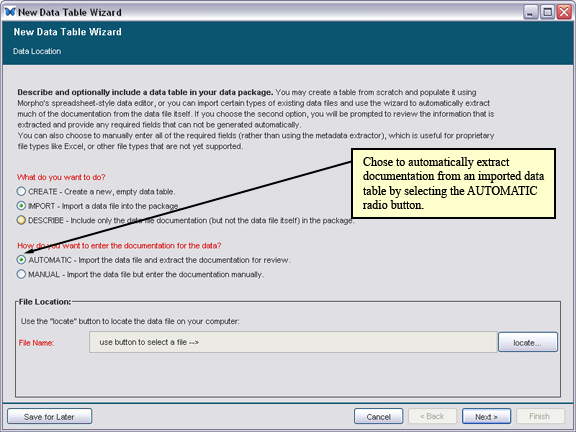
\includegraphics[width=0.7\textwidth]{images/wizard-table-import-automatic.jpg}
  \caption{Automatically extract documentation from the imported data
    table and present it for review.}
  \label{fig:wizard-table-import-automatic}
\end{figure}

When you choose to automatically extract documentation, the Data Table
wizard displays the imported data table and prompts you to specify a
table name, description, and additional information that helps Morpho
import the documentation correctly
(\autoref{fig:wizard-table-import-extract}). 

If the first few rows of the data table are blank, you can choose to
begin importing at a row other than ``1'' by specifying a later start
row in the ``Start import at row'' field.

If the first row contains column labels (as in the example above), then
check the box beside the ``Column labels are in starting row'' setting.
Click Next to continue (\autoref{fig:wizard-table-delimiter}).

\begin{figure}
  \centering
    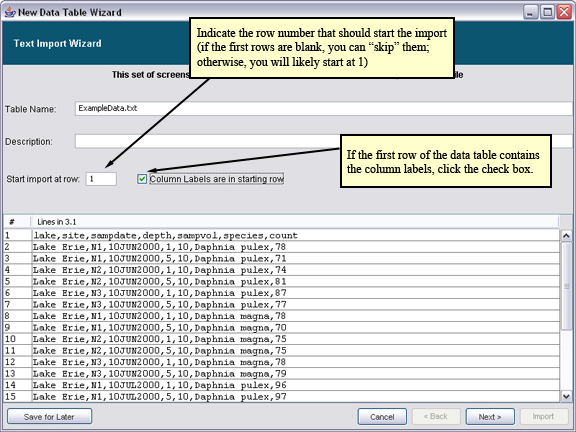
\includegraphics[width=0.7\textwidth]{images/wizard-table-import-extract.jpg}
  \caption{An example of importing a data table and automatically
    extracting the documentation. Your data may look significantly
    different from the sample data displayed.}
  \label{fig:wizard-table-import-extract}
\end{figure}

\begin{figure}
  \centering
    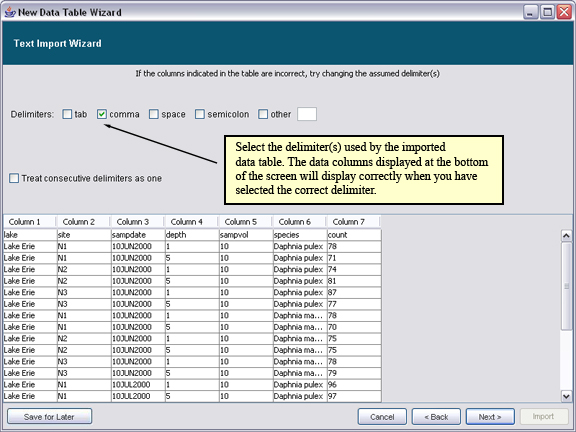
\includegraphics[width=0.7\textwidth]{images/wizard-table-delimiter.jpg}
  \caption{Selecting the data table delimiters.}
  \label{fig:wizard-table-delimiter}
\end{figure}

Select one or more delimiter, or specify a new delimiter in the
``other'' field. The data columns displayed at the bottom of the screen
will display correctly when you have selected the correct delimiter or
combination of delimiters. To indicate that consecutive delimiters be
used as one, check the box beside ``Treat consecutive delimiters as
one.'' Click ``Next'' to review the extracted documentation
(\autoref{fig:wizard-table-attribute-extraction}).

\begin{figure}
  \centering
    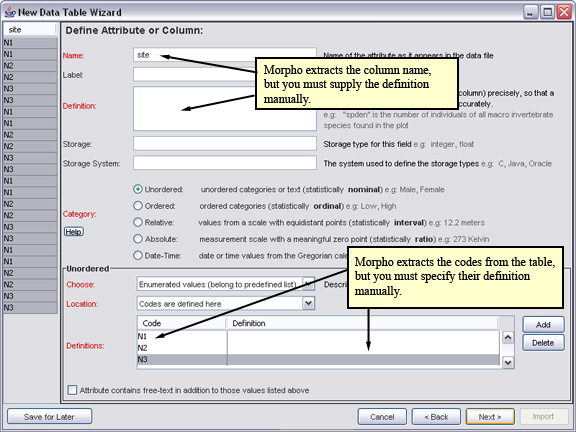
\includegraphics[width=0.7\textwidth]{images/wizard-table-attribute-extraction}
  \caption{Reviewing extracted documentation.}
  \label{fig:wizard-table-attribute-extraction}
\end{figure}

Note that Morpho automatically places extracted codes in the table under
``Code'', but you must provide the code definitions. You must also
provide column definitions (Morpho does not do this automatically).
Before clicking Next to review the next column of extracted
documentation, examine the documentation to make sure all category,
unit, and other documentation is correct. You can add to the
documentation or change erroneous documentation in the fields provided.
For more information about the fields in the Data Table wizard, please
see \autoref{sec:table-documenting}.

\subsection[Adding Other Data Table Types]{Adding Other Data Table Types (E.g. 
Excel, Mathematica, HTML, or XML)} \label{sec:table-other-types}

Data stored in proprietary binary formats such as Excel, Mathematica, or
Word documents, can be
added to data packages using the Data Table wizard. Although the current
version of Morpho does not support displaying the content of most proprietary
formats, such files can still be documented using the Morpho wizards and
saved to a data package. If your data package contains data files stored
in a proprietary format, you can view the data by exporting the data
package to a convenient directory and using the creator application
(e.g., Excel or Word) to open and view the data.

Note that applications such as Excel and Microsoft Access also permit
you to export data as a simple delimited file, which can be imported
into Morpho and displayed. For example, to export Microsoft Access
tables as delimited text files, click each data table and export it as a
text file (under File $>$ Export...). If you have data in an Excel
workbook, simply save each worksheet as a text file using ``Save As''
and choosing the ``Text (Tab-delimited)'' format from the ``Save as
type'' menu. Note that chart objects in Excel cannot be saved as text
files. 

To add a proprietary file to a data package:
\begin{enumerate}
  \item Open the data package to which you wish to save the data file.
    From the Data menu at the top of the Data Package screen, select
    Create/Import new Data Table. The Data Table wizard opens.
  \item In the Data Table wizard, select ``Import'' and ``Manual''
    (\autoref{fig:wizard-table-filelocation}). Click the locate button
    to select the file to import. Click Next.
  \item In the Data Table wizard's File Format screen, select ``Non-text
    or proprietary format that is externally defined,'' and then choose
    the appropriate format from the list
    (\autoref{fig:wizard-table-import-nontext}), or ``other'' if the
    data format does not appear in the list (e.g the MIME type or a short
    description). 
    Note: It is often preferable to import image files as ``other entities'' 
    as described in \autoref{sec:importing-other-entities}.
\end{enumerate}

\begin{figure}
  \centering
    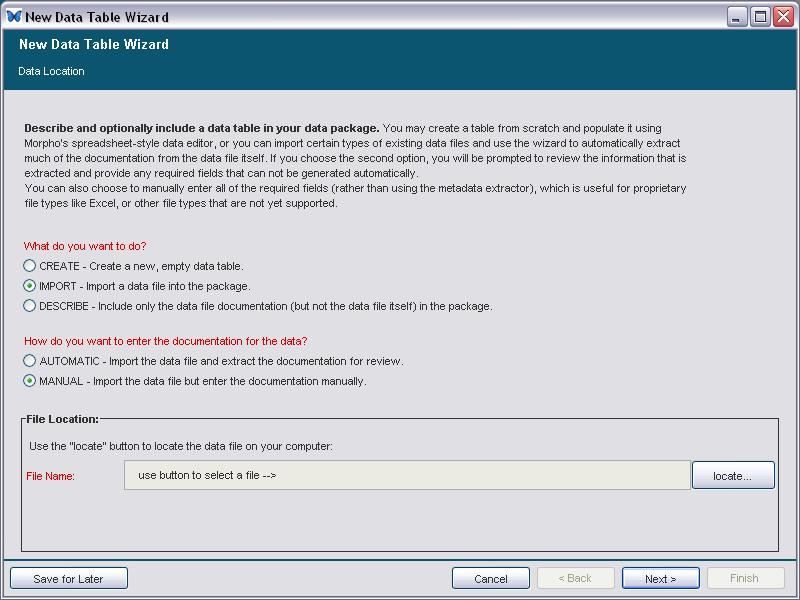
\includegraphics[width=0.7\textwidth]{images/wizard-table-filelocation.jpg}
  \caption{Adding an Excel or other proprietary data file to a
    data package.}
  \label{fig:wizard-table-filelocation}
\end{figure}

\begin{figure}
  \centering
    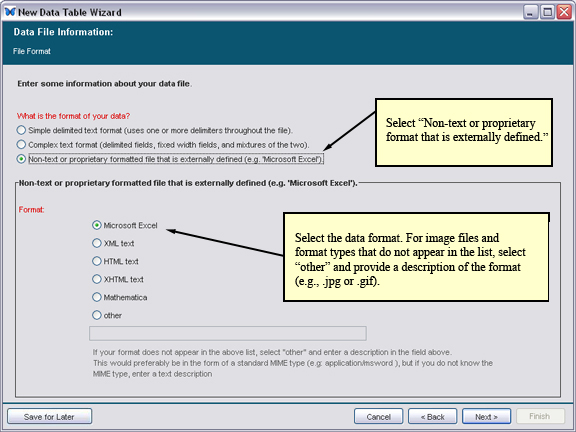
\includegraphics[width=0.7\textwidth]{images/wizard-table-import-nontext.jpg}
  \caption{Adding a non-text or proprietary file to a data package.}
  \label{fig:wizard-table-import-nontext}
\end{figure}

Once you have identified the data file and its format, use the Data
Table wizard to document it just as you would a delimited text file. For
more information about using the Data Table Wizard to document data, see
\autoref{sec:table-documenting}.

\begin{shaded}
  \textbf{NOTE} Complex, geospatially indexed images can be included in
  data packages and described in EML 2.0 and newer versions using the
  ``spatialRaster'' or ``spatialVector'' entity modules. However, the
  Morpho wizards currently do not support adding documentation to these
  modules. For more information about EML, please see the Guide to EML.
\end{shaded}

\subsection[Adding Other Data Entities]{Adding Other Data Entities (E.g. 
binary files, images, PDFs)} \label{sec:importing-other-entities}

While the Data Table import wizard can be used to import binary and proprietary 
data files, it should only used when the file contains a describable data structure 
such that attribute-level documentation can be entered (as is the case with a 
tabular Excel worksheet). Data files that do not adhere to an entity/attribute 
structure (e.g. digitized field notes in PDF, specimen jpeg images) should be 
imported as ``other entities''.

To add other data entities to a data package:
\begin{enumerate}
  \item Open the data package to which you wish to save the data file.
    From the Data menu at the top of the Data Package screen, select
    ``Import Other Data''.
  \item Select the file to be imported (\autoref{fig:import-other-entity-location}). 
  Click the ``locate'' button to select the file to import.
  \item Click ``Ok''.
  Basic file metadata (file type and file size) will be collected automatically .
\end{enumerate}

\begin{figure}
  \centering
    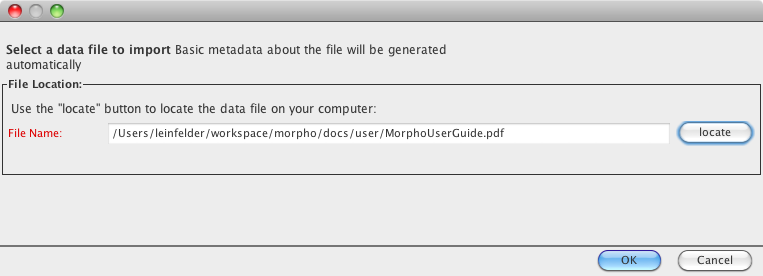
\includegraphics[width=0.7\textwidth]{images/import-other-entity-location.png}
  \caption{Adding a binary or non-tabular data file to a data package.}
  \label{fig:import-other-entity-location}
\end{figure}

\subsection[Converting Other Entities to Data Tables]{Converting 
Other Entities to Data Tables}
\label{sec:converting-other-entities}

If tabular data has previously been added to a Data Package as 
an ``other entity'' (e.g. using the KNB online data registry) it can be converted
to a Data Table using the Data Table wizard. Attribute-level metadata
is entered in the same way as it is when importing a new data table,
but after the conversion, the old data entity will need to be explicitly removed 
from the data package.

To convert an other entity to a data table:
\begin{enumerate}
  \item From the Data menu at the top of the Data Package screen, select
    ``Convert Data to Table''.
  \item The New Data Table Wizard will launch with the Data Location fields
  pre-populated (\autoref{fig:convert-other-entity-location}). 
  \item Click ``Next'' to continue through the Data Table import wizard as described in
  \autoref{sec:table-import}
  \item When the wizard has completed, the original entity can be removed and the new
  table will be unaffected. See \autoref{sec:deleting-current-data} for instructions on removing
  data entities.
\end{enumerate}

\begin{figure}
  \centering
    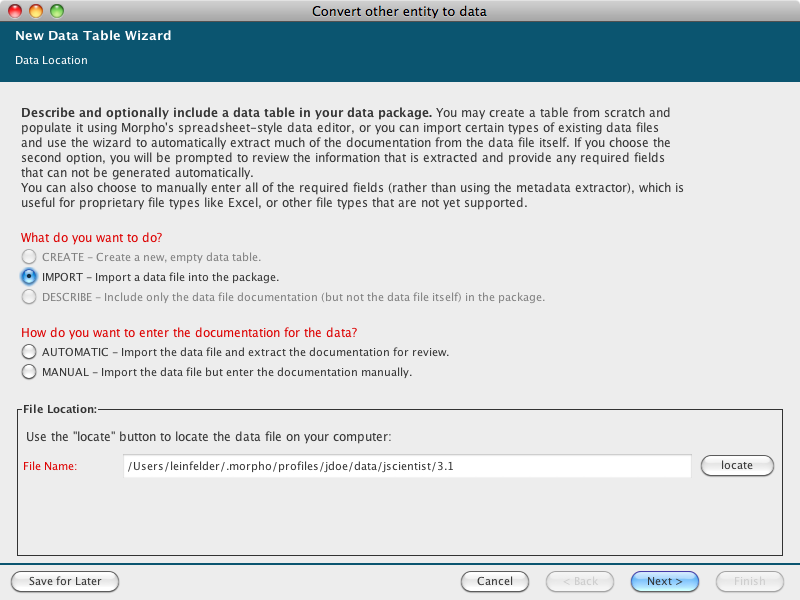
\includegraphics[width=0.7\textwidth]{images/convert-other-entity-location.png}
  \caption{Converting an other entity to a data table.}
  \label{fig:convert-other-entity-location}
\end{figure}

\subsection[Replacing Data]{Replacing Data}
\label{sec:replacing-data}

Existing Data Tables can have their data replaced while still 
preserving the original metadata that was so meticulously entered during the initial import.
This allows a data table to be described before the data is fully cleaned and finalized, 
thereby making Morpho useful for active data management.

\begin{shaded}
  \textbf{NOTE} When replacing the data content of a table, close attention must me paid to the table structure. 
  The order and number of columns/attributes must remain the same or else the metadata will not match the new data.
\end{shaded}

To replace a data file:
\begin{enumerate}
  \item From the Data menu at the top of the Data Package screen, select
    ``Replace Current Data''.
  \item Select the new data file to import (\autoref{fig:replace-data-location}). 
  \item Enter an optional name for the entity (the file name will be used if this is omitted).
  \item Click ``Ok''. The file size, and row count metadata will be recalculated automatically 
  and saved in the entity metadata.
\end{enumerate}

\begin{figure}
  \centering
    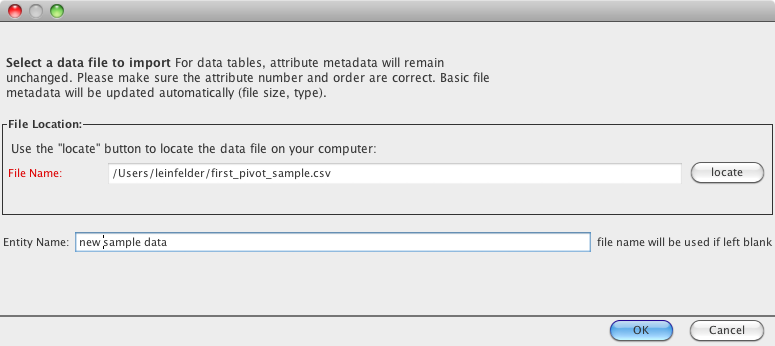
\includegraphics[width=0.7\textwidth]{images/replace-data-location.png}
  \caption{Replacing a data file.}
  \label{fig:replace-data-location}
\end{figure}

\subsection[Exporting Data Entities]{Exporting Data Entities}
\label{sec:exporting-entities}

In addition to the Data Package Export feature (see \autoref{sec:exporting-data-packages}),
individual data entities can be exported. This is useful for binary or proprietary 
data files that cannot be displayed inside Morpho.

To export data entities:
\begin{enumerate}
  \item Open the data package containing the data file.
  \item From the Data menu at the top of the Data Package screen, 
  select ``Export Data''.
  \item Specify a directory where the data will be exported.
   For organization, a subdirectory with the package ID will 
   automatically be created in the directory you select.
\end{enumerate}

\subsection{Saving Incomplete Data Tables }

Saving an incomplete data table description in the Data Table Wizard is
similar to saving incomplete Data Packages. For more information, please
see \autoref{sec:dp-saveforlater}.

\subsection{Recovering Incomplete Data Tables}

Recovering an incomplete data table description is similar to Recovering
Incomplete Data Packages. For more information, please see
\autoref{sec:dp-recover}.

\subsection{Working with Data Tables and Documentation}
\label{sec:working-with-data}

Once data have been created (or imported into Morpho) and documented,
you can edit and/or manipulate the data using the options under the
\nameref{sec:menu-data} and \nameref{sec:menu-edit}. These options allow
you to edit the data table documentation, to sort the data, to delete
rows or columns of data, or to insert new rows or columns. You can also
access these menu options by right-clicking a row or column in the data
table.

\begin{itemize}
  \setlength{\parskip}{1pt}
  \item \nameref{sec:edit-table-sort}
  \item \nameref{sec:edit-table-rowcol}
  \item \nameref{sec:edit-table-col-doc}
  \item \nameref{sec:edit-table-col-copypaste}
  \item \nameref{sec:edit-table-access}
  \item \nameref{sec:edit-table-revert}
  \item \nameref{sec:deleting-current-data}
\end{itemize}

\subsubsection{Sorting Table Rows}
\label{sec:edit-table-sort}

To sort the rows of a data table, select the column which you would like
to sort by, and click ``Sort by Selected Column''
(\autoref{fig:edit-table-sort-column}). Morpho rearranges the rows of
data according to the value of the selected column. The rows themselves
remain unchanged, only repositioned.

\begin{figure}
  \centering
    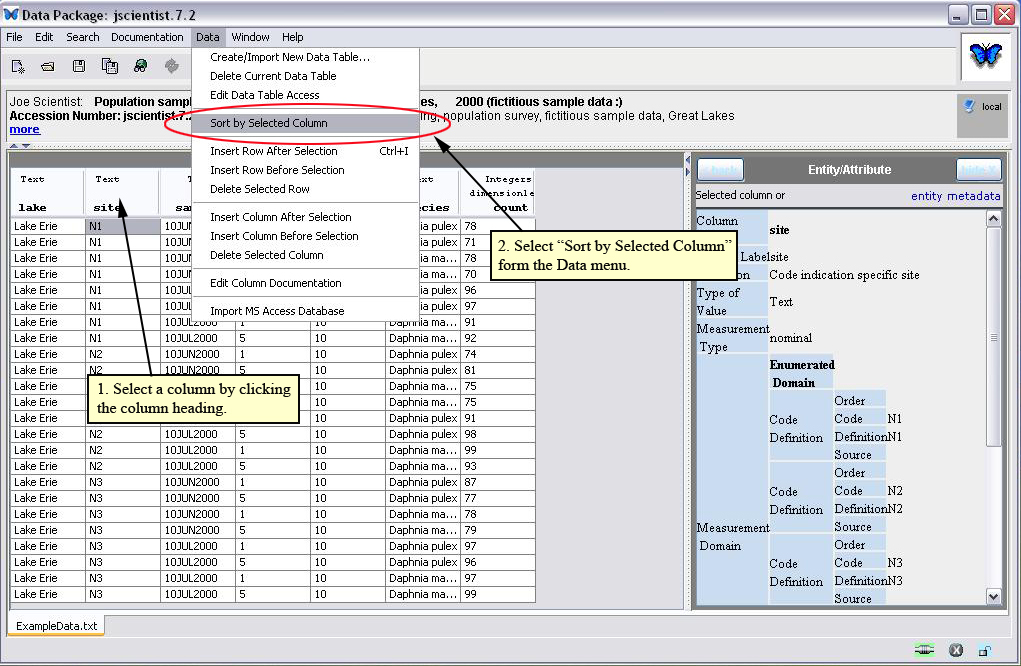
\includegraphics[width=0.7\textwidth]{images/edit-table-sort-column.jpg}
  \caption{Sorting a data table.}
  \label{fig:edit-table-sort-column}
\end{figure}

\subsubsection{Inserting and Deleting Rows and Columns}
\label{sec:edit-table-rowcol}

Morpho can insert and delete rows and columns of data (much like
Microsoft Excel does). To insert a row/column, select the row/column
adjacent to where you wish to insert the new cells. To select a column,
click the column header or any item in the column. To select a row,
click any item in the row. New rows and columns can be positioned on
either side of the selected item (\autoref{fig:edit-table-row-delete}).
Inserting a new row simply creates a new, empty row (you can also create
a new row by pressing CTRL-I). When you choose to insert a column,
Morpho prompts you to specify attribute metadata for that column. After
you have entered the metadata, Morpho creates the empty column for the
corresponding data.

\begin{figure}
  \centering
    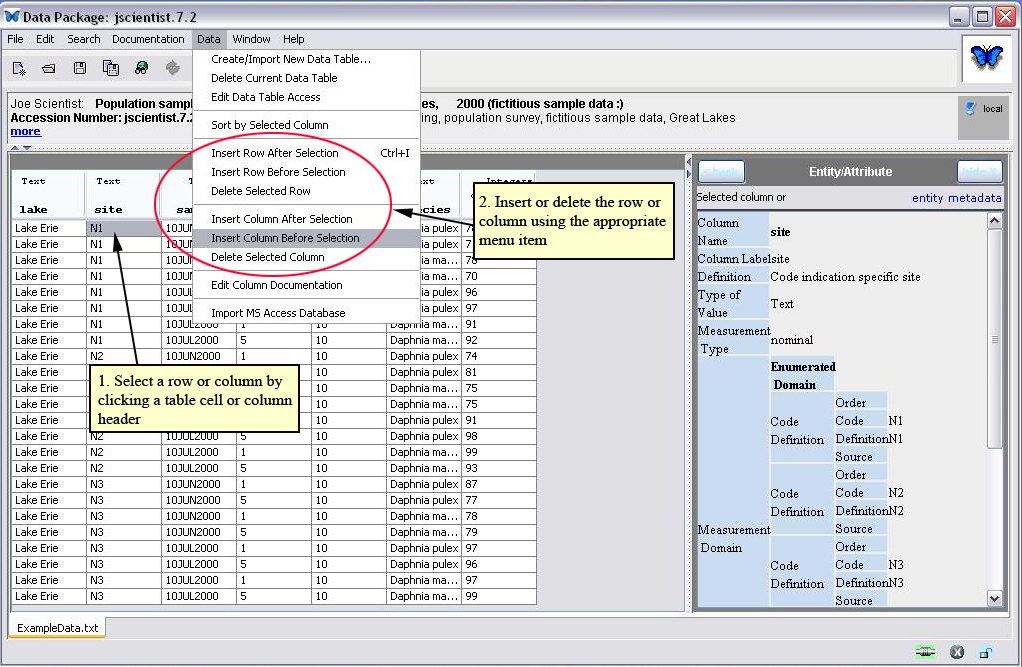
\includegraphics[width=0.7\textwidth]{images/edit-table-row-delete}
  \caption{Inserting and deleting rows and columns.}
  \label{fig:edit-table-row-delete}
\end{figure}

\subsubsection{Editing Column Documentation}
\label{sec:edit-table-col-doc}

To edit documentation entered using the Data Table Wizard, or to add
additional documentation to a table column, select the column by
clicking the column header or a cell beneath it and then select ``Edit
Column Documentation'' from the Data menu. 

Morpho will display the column documentation
(\autoref{fig:edit-table-column-documentation}).  

\begin{figure}
  \centering
    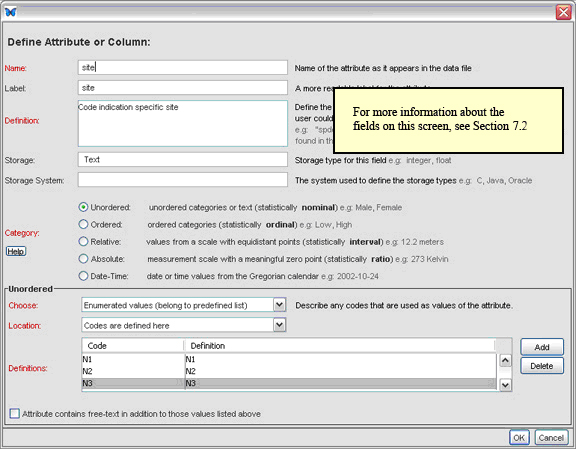
\includegraphics[width=0.7\textwidth]{images/edit-table-column-documentation.jpg}
  \caption{Adding or editing documentation to a table column.}
  \label{fig:edit-table-column-documentation}
\end{figure}

\subsubsection{Cutting, Copying, and Pasting Table Data}
\label{sec:edit-table-col-copypaste}

Cut, copy, and paste functions can be accessed under the ``Edit'' menu
(\autoref{fig:edit-table-column-copy-paste}) or using keyboard
shortcuts: Ctrl+X for cut, Ctrl+V for paste, and Ctrl+C for copy. These
functions work just as they do in Microsoft applications like Word and
Excel.

\begin{figure}
  \centering
    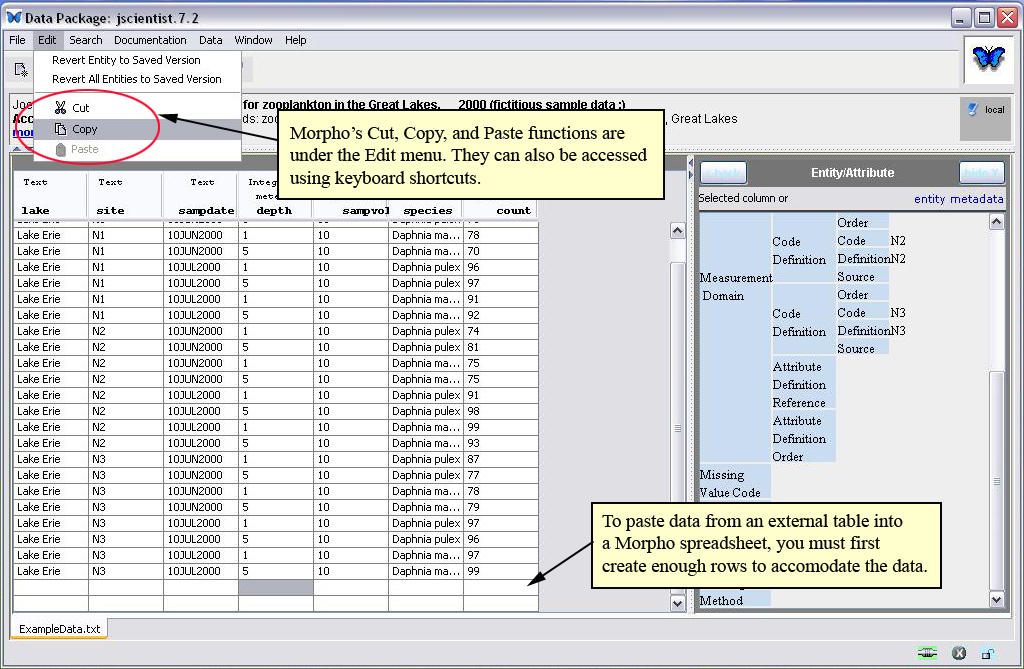
\includegraphics[width=0.7\textwidth]{images/edit-table-column-copy-paste.jpg}
  \caption{Cut, copy, and paste in Morpho.}
  \label{fig:edit-table-column-copy-paste}
\end{figure}


Use cut, copy, and paste to relocate or delete rows and columns, or to
paste data from an external data source (such as an Excel file) into
Morpho. Note that Morpho does not automatically add new rows to the data
table when information is pasted. Thus, if you want to add data by
pasting them into Morpho's spreadsheet editor, you must first create
additional table rows to accommodate them. To create new rows, select
the last row in the data table and press CTRL-I to insert a new empty
row (or use the insert option in the Data or right-click menus). After
creating the required number of new rows, select the top empty row and
paste the new data. 

\begin{shaded}
  \textbf{NOTE} The default delimiter used when copying/pasting from
  Excel is a tab. If existing data uses a different delimiter (e.g., a
  comma), then the pasted data will end up in the first cell.
\end{shaded}

\subsubsection{Setting Access Control} \label{sec:edit-table-access}

Initially, the \hyperref[sec:wizard-dp-access]{access information
specified for the data package} applies to all data tables that
are imported to the package. To specify different permissions for a 
specific data table after the data has been imported,
select ``Edit Data Table Access'' from the Data menu
(\autoref{fig:edit-table-access}).

\begin{figure}
  \centering
    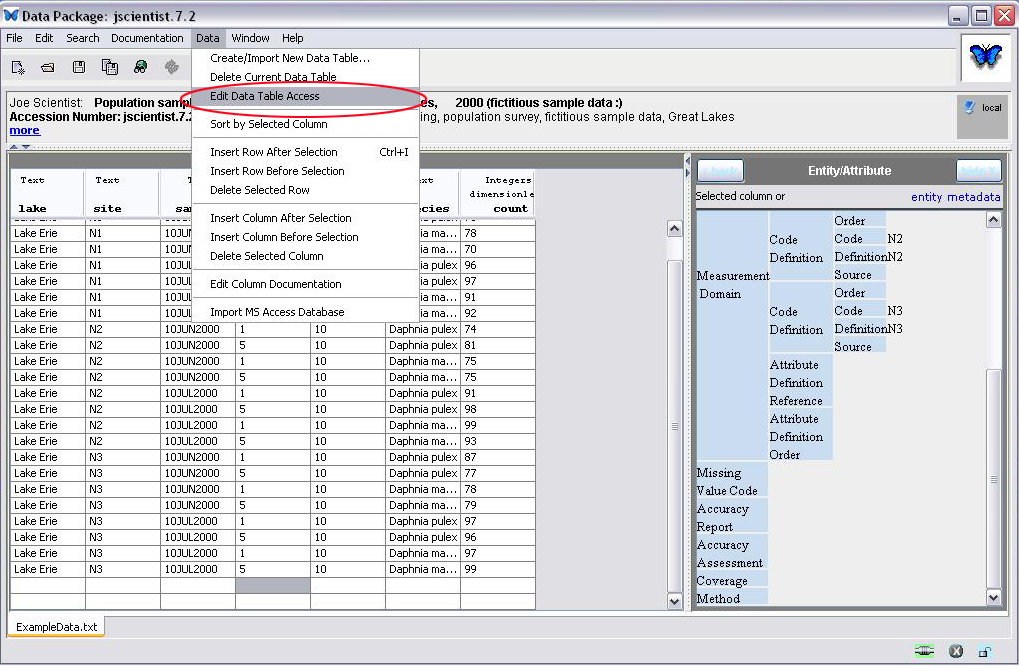
\includegraphics[width=0.7\textwidth]{images/edit-table-access.jpg}
  \caption{Editing the data table access.}
  \label{fig:edit-table-access}
\end{figure}

The access customization screen opens
(\autoref{fig:dialog-access-table}), allowing you to specify read,
write, change permissions access to individual users or groups. 
The settings will apply only to this single table, and will override
the settings that were originally inherited from the data package. For more
information about access permissions, see
\nameref{sec:wizard-dp-access}.

\begin{figure}
  \centering
    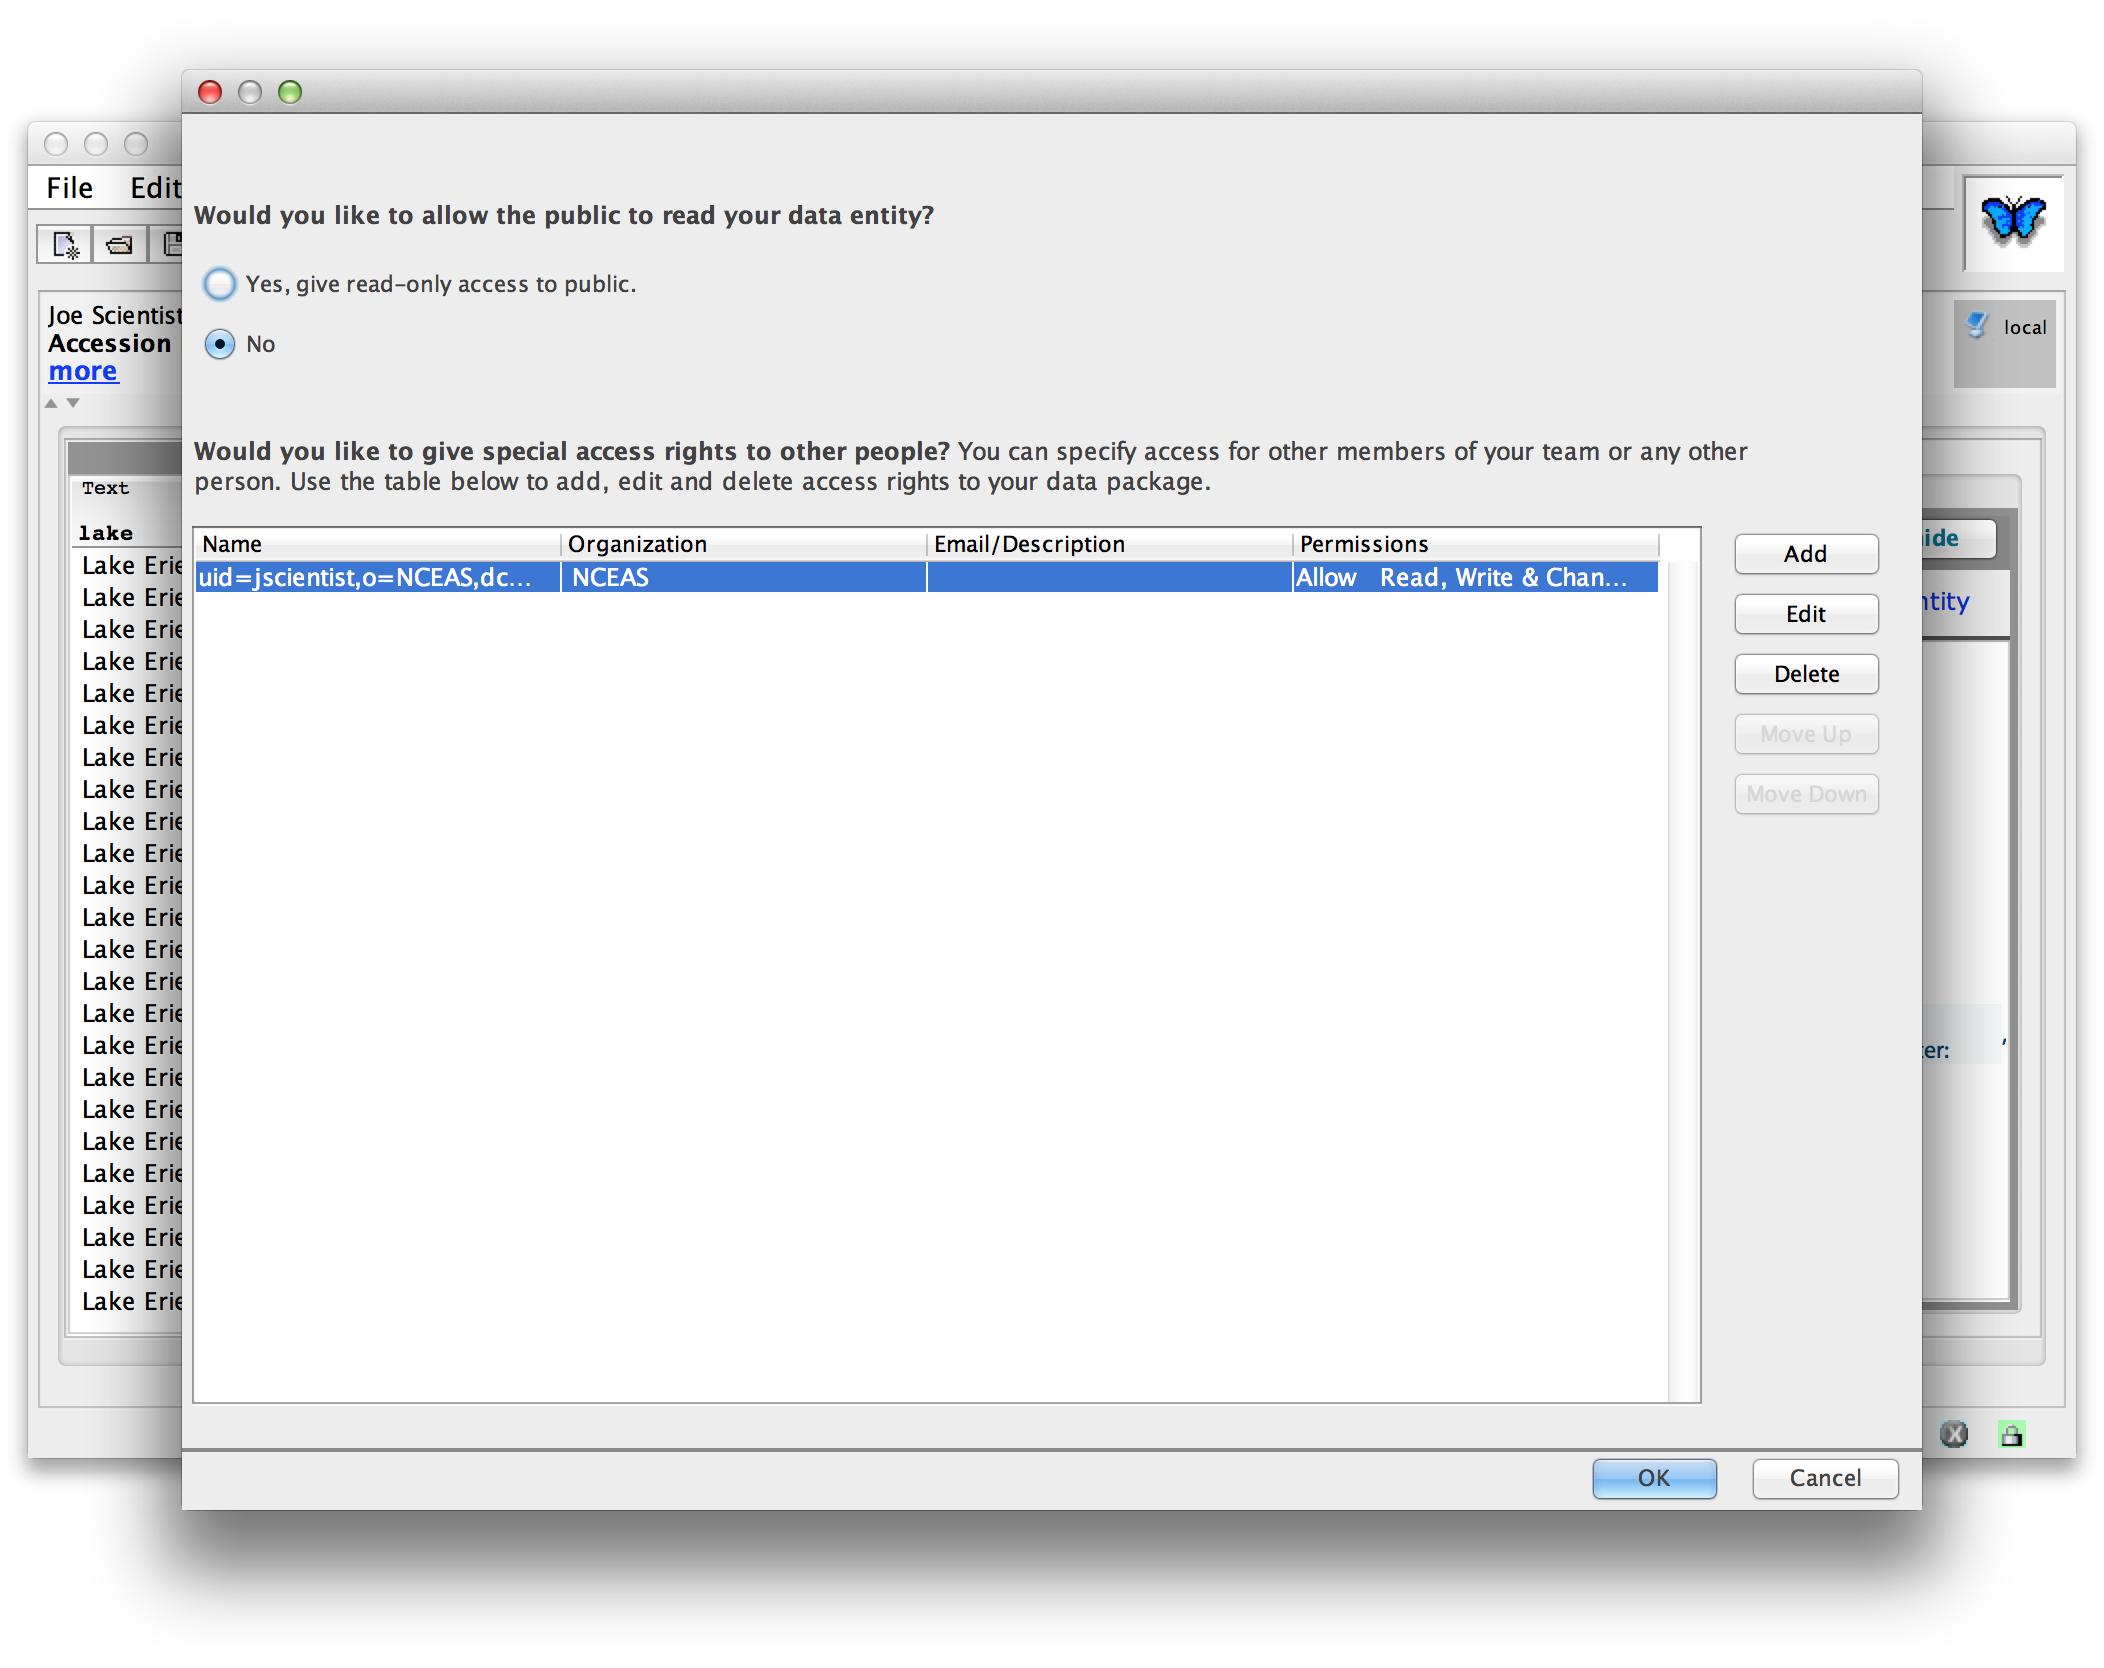
\includegraphics[width=0.7\textwidth]{images/dialog-access-table.png}
  \caption{Setting access permissions for individual data objects.}
  \label{fig:dialog-access-table}
\end{figure}

\subsubsection{Reverting (Undoing Changes)}
\label{sec:edit-table-revert}

You can undo changes you have made to one or more of the tables in your
data package as long as you have not saved the data package since making
the changes. To undo changes to the displayed table, select ``Revert
Entity to Saved Version'' from the Edit menu. All changes made since the
last time you saved the data package will be reversed. 

To undo changes made to all of the tables in the data package, select
``Revert All Entities to Saved Version'' from the Edit menu.

\subsubsection{Deleting Data}
\label{sec:deleting-current-data}

Data Tables and Entities can be removed from the Data Package 
using the ``Data $>$ Delete Current Data'' menu option. Before invoking 
this command, select the tab for the data that should be removed.

To undo this action, simply close the data package without saving it 
and then reopen the package.
